
\documentclass[11pt]{article}
\usepackage[margin=1in]{geometry}
\usepackage{amsmath}
\usepackage{amssymb}
\usepackage{booktabs}
\usepackage{graphicx}
\usepackage{float}
\usepackage{caption}
\captionsetup{font=small}
\title{Unsupervised Human Activity Recognition using Bayesian Hidden Markov Models}
\author{Albert Cai \\ Jiashu Li}
\date{March 2026}

\begin{document}
\maketitle

\begin{abstract}
We study unsupervised human activity recognition on the UCI smartphone HAR dataset using finite-state Gaussian hidden Markov models. Following our proposal, we compare a classical EM-trained Gaussian HMM against a Bayesian HMM with Dirichlet priors on transition probabilities and Normal-Inverse-Wishart priors on Gaussian emissions. A toy-data sanity check verifies that the Bayesian sampler can recover latent state structure and transition dynamics from synthetic sequences with known parameters. On the HAR benchmark, we reduce the 561 engineered features to eight principal components and treat each subject as an independent sequence. The EM baseline clustered the held-out HAR subjects slightly better, but the Bayesian model remained competitive while exposing uncertainty over persistence. The resulting analysis highlights both the benefits and the practical tradeoffs of Bayesian parameter uncertainty in sequential clustering problems.
\end{abstract}

\section{Introduction}
Human activity recognition (HAR) aims to infer behaviors such as walking, sitting, and standing from wearable sensor streams. Most modern HAR systems are supervised, but in many realistic deployments labels are expensive, incomplete, or unavailable. This makes probabilistic latent-variable models attractive because they can discover structure directly from noisy sequential measurements while also modeling temporal dependence between activities.

This project asks whether a Bayesian hidden Markov model (HMM) offers a more robust unsupervised HAR pipeline than a classical maximum-likelihood HMM. The course motivation is a natural fit: HMMs provide a compact directed graphical model, exact inference through forward-backward recursions, and a clean Bayesian extension through conjugate priors and MCMC.

\section{Model Overview}
Figure~\ref{fig:diagram} shows the sequential model. For each subject-specific sequence, latent states $z_t \in \{1,\dots,K\}$ evolve as a first-order Markov chain and emit reduced-dimensional sensor vectors $x_t \in \mathbb{R}^d$:
\begin{align}
p(z_1) &= \pi_{z_1}, \\
p(z_t \mid z_{t-1}) &= A_{z_{t-1}, z_t}, \\
x_t \mid z_t = k &\sim \mathcal{N}(\mu_k, \Sigma_k).
\end{align}
We fix $K=6$ hidden states to match the six activities in the benchmark and set $d=8$ principal components after standardizing the original 561 features. This PCA projection retains 78.7\% of the variance while keeping full-covariance Gaussian inference numerically stable.

For the EM baseline, we maximize the observed-data likelihood with exact E-steps from forward-backward and closed-form M-steps for $\pi$, $A$, $\mu_k$, and $\Sigma_k$. For the Bayesian model, we use
\begin{align}
\pi &\sim \text{Dirichlet}(\alpha_\pi \mathbf{1}), \\
A_k &\sim \text{Dirichlet}(\alpha_A \mathbf{1}), \\
(\mu_k, \Sigma_k) &\sim \text{NIW}(m_0, \kappa_0, \Psi_0, \nu_0),
\end{align}
and alternate three Gibbs updates: sampling initial and transition probabilities from Dirichlet posteriors, sampling emission parameters from NIW posteriors, and sampling latent state sequences with forward-filtering backward-sampling.

\begin{figure}[H]
\centering
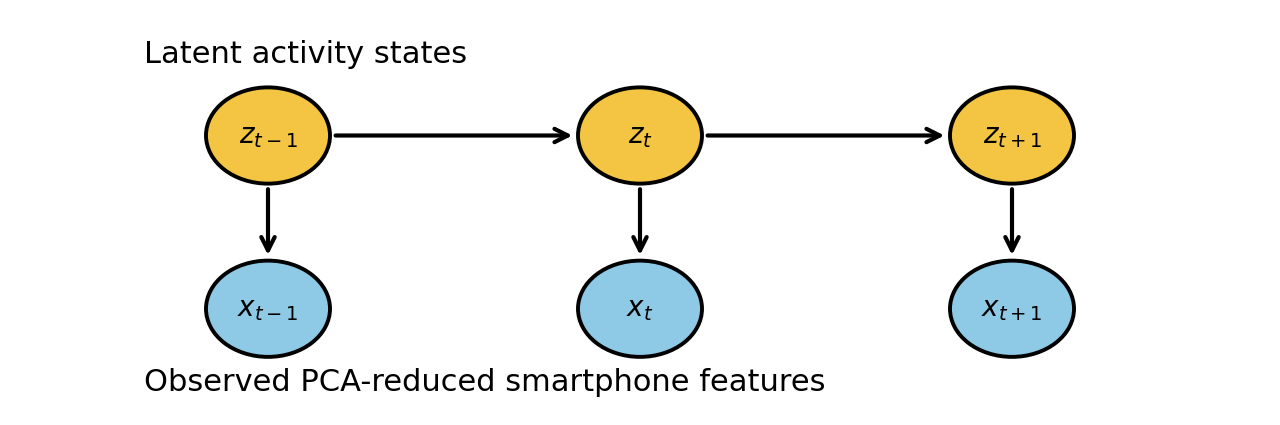
\includegraphics[width=0.82\linewidth]{figures/hmm_diagram.png}
\caption{Graphical sketch of the Gaussian HMM used for HAR. Yellow nodes are latent activity states and blue nodes are observed PCA-reduced sensor features.}
\label{fig:diagram}
\end{figure}

\section{Experimental Setup}
The UCI HAR dataset contains 10,299 sliding-window observations collected from 30 subjects performing six activities. We use the provided train/test split, standardize the 561 engineered features using training-set statistics, project onto eight principal components, and treat each subject as one sequence. Evaluation is unsupervised: we train without labels and then compare inferred states to true activities with adjusted Rand index (ARI), normalized mutual information (NMI), and an aligned accuracy computed after Hungarian matching. We also report held-out log-likelihood and a simple robustness check where Gaussian noise is added to the test features.

Before touching the real dataset, we run a toy sanity check with a three-state Gaussian HMM whose true parameters are known. This lets us test whether the sampler recovers state sequences and transition structure at all.

\section{Results}
\subsection{Toy-data sanity check}
The synthetic experiment confirms that the Bayesian HMM can recover latent structure from data generated by the model family. On held-out synthetic sequences, the EM baseline obtained ARI 0.477 and aligned accuracy 0.581, while the Bayesian HMM obtained ARI 0.533 and aligned accuracy 0.675.

\begin{figure}[H]
\centering
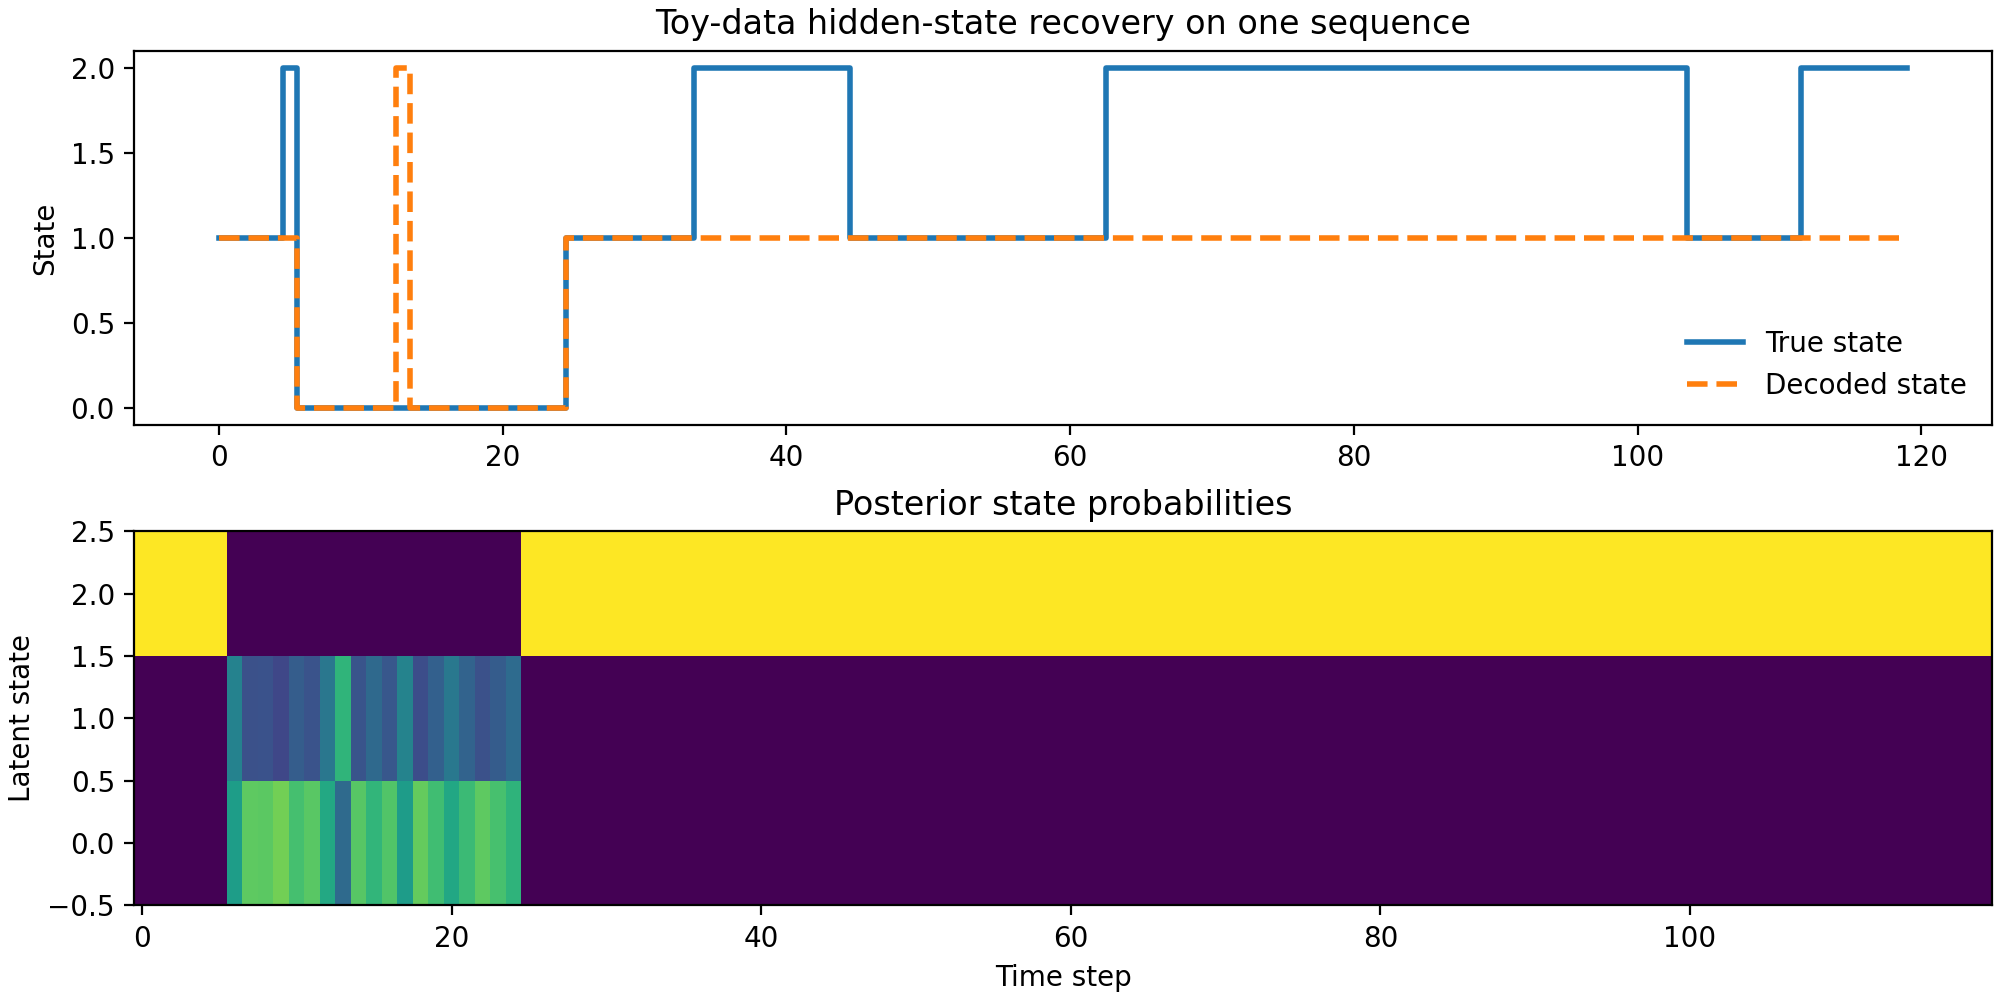
\includegraphics[width=0.88\linewidth]{figures/toy_state_recovery.png}
\caption{Toy-data sanity check. Top: true versus decoded latent states for one sequence. Bottom: posterior state probabilities from the Bayesian HMM.}
\end{figure}

\begin{figure}[H]
\centering
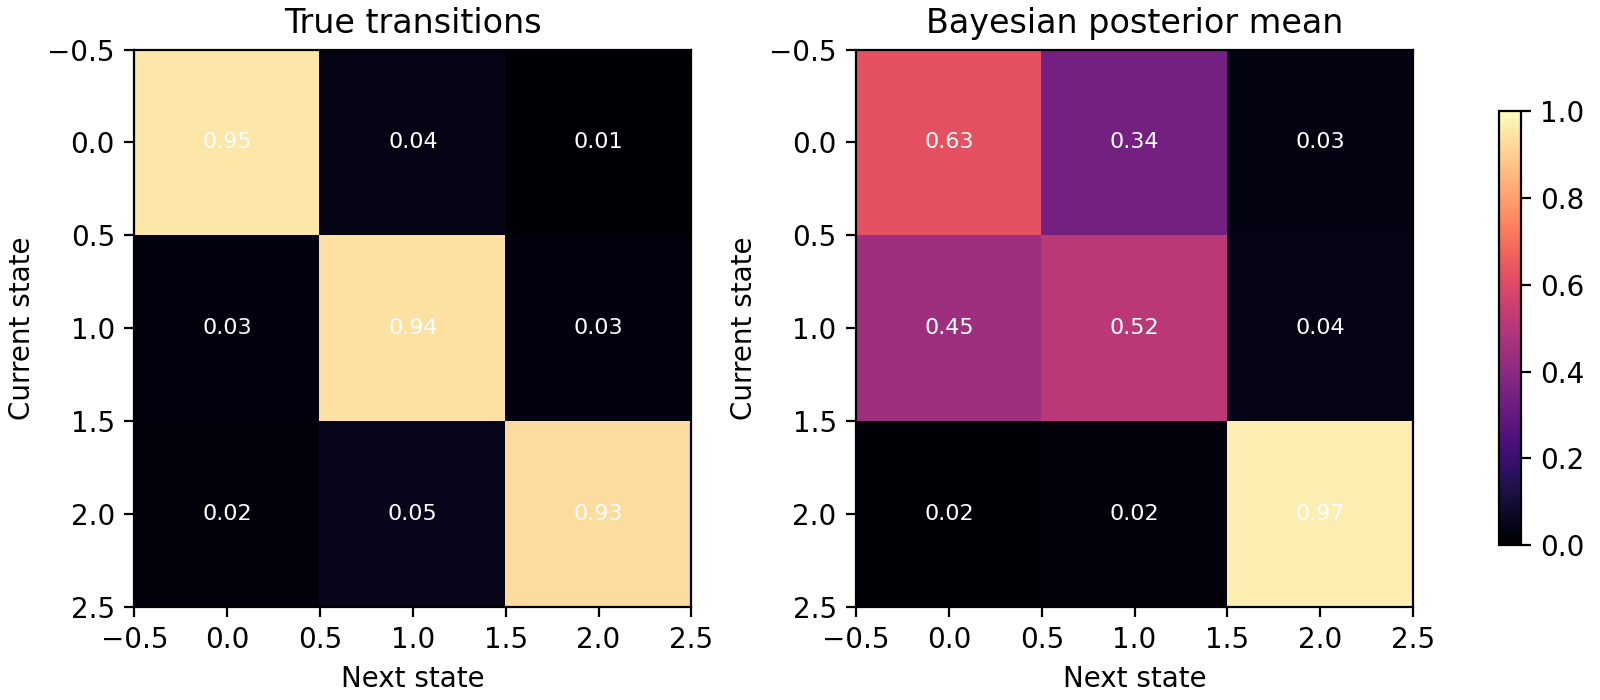
\includegraphics[width=0.76\linewidth]{figures/toy_transition_recovery.png}
\caption{True toy transition matrix compared with the Bayesian posterior-mean transition matrix.}
\end{figure}

\subsection{UCI HAR comparison}
Table~\ref{tab:main} summarizes the main quantitative comparison. The EM model achieved test ARI 0.301 and NMI 0.497, while the Bayesian model achieved test ARI 0.300 and NMI 0.493. Held-out log-likelihood was -22686.1 for EM and -22667.7 for the Bayesian posterior-mean model.

\begin{table}[H]
\centering
\begin{tabular}{lcccc}
\toprule
Model & Test ARI & Test NMI & Test aligned acc. & Test log-likelihood \\
\midrule
EM-HMM & 0.301 & 0.497 & 0.448 & -22686.1 \\
Bayesian HMM & 0.300 & 0.493 & 0.447 & -22667.7 \\
\bottomrule
\end{tabular}
\caption{Held-out clustering and likelihood comparison on UCI HAR.}
\label{tab:main}
\end{table}

\begin{figure}[H]
\centering
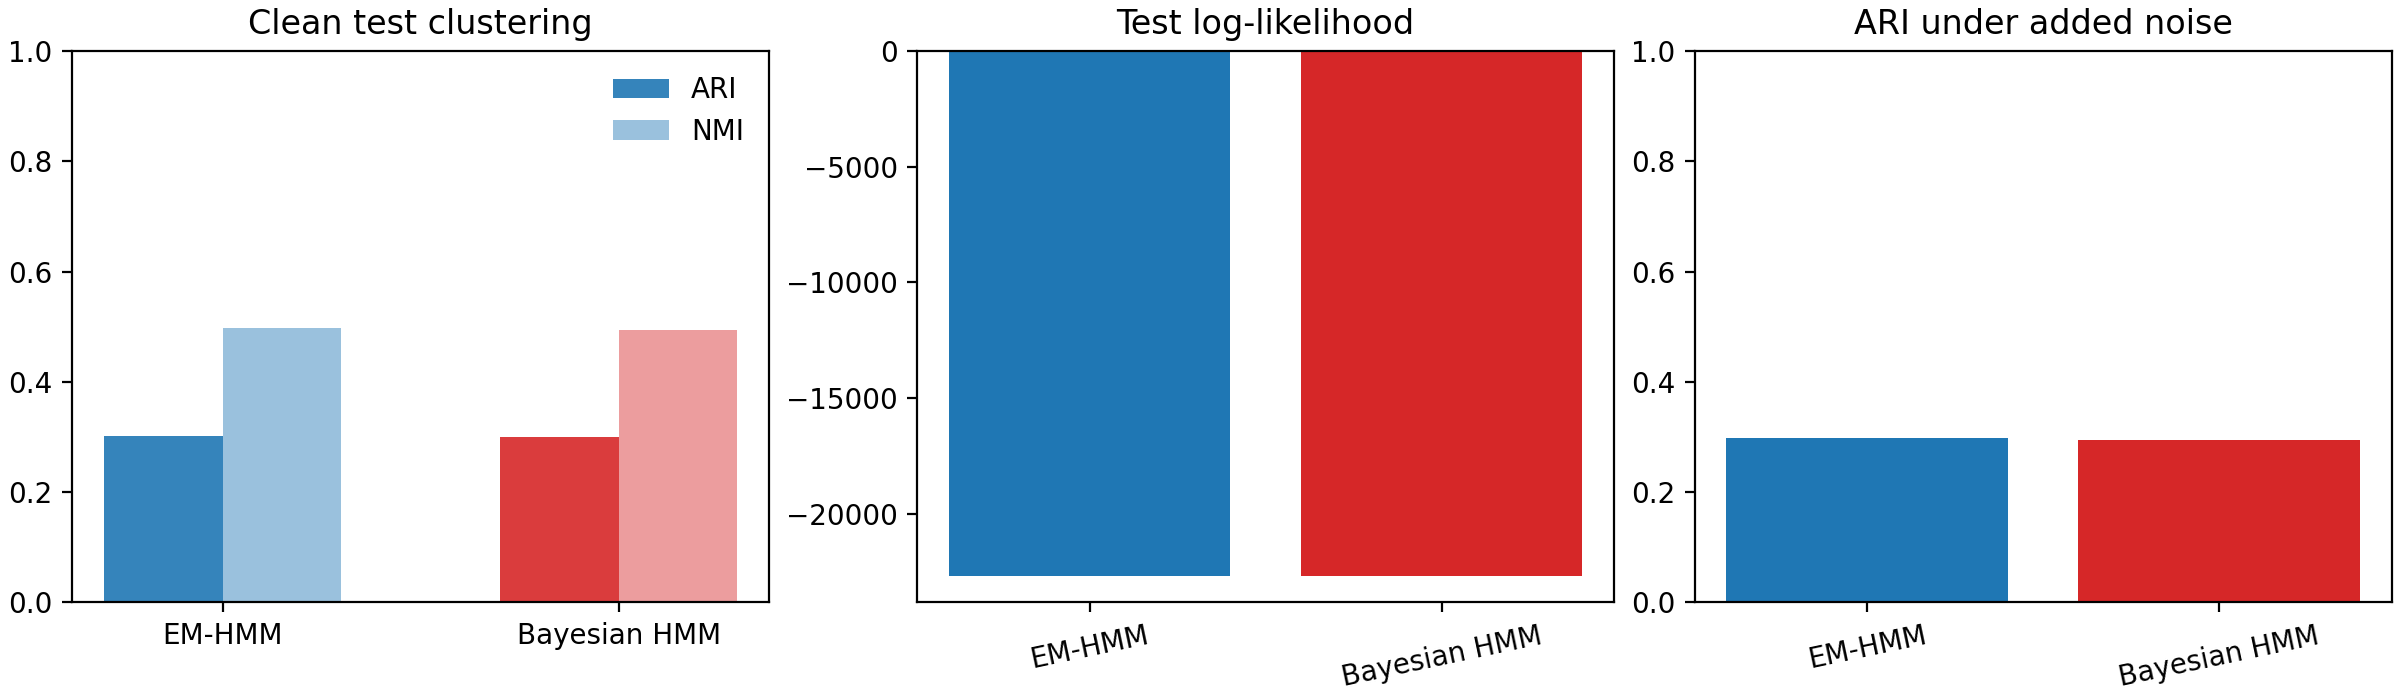
\includegraphics[width=\linewidth]{figures/har_model_comparison.png}
\caption{HAR comparison across clean clustering quality, held-out log-likelihood, and robustness under added Gaussian noise.}
\end{figure}

\begin{figure}[H]
\centering
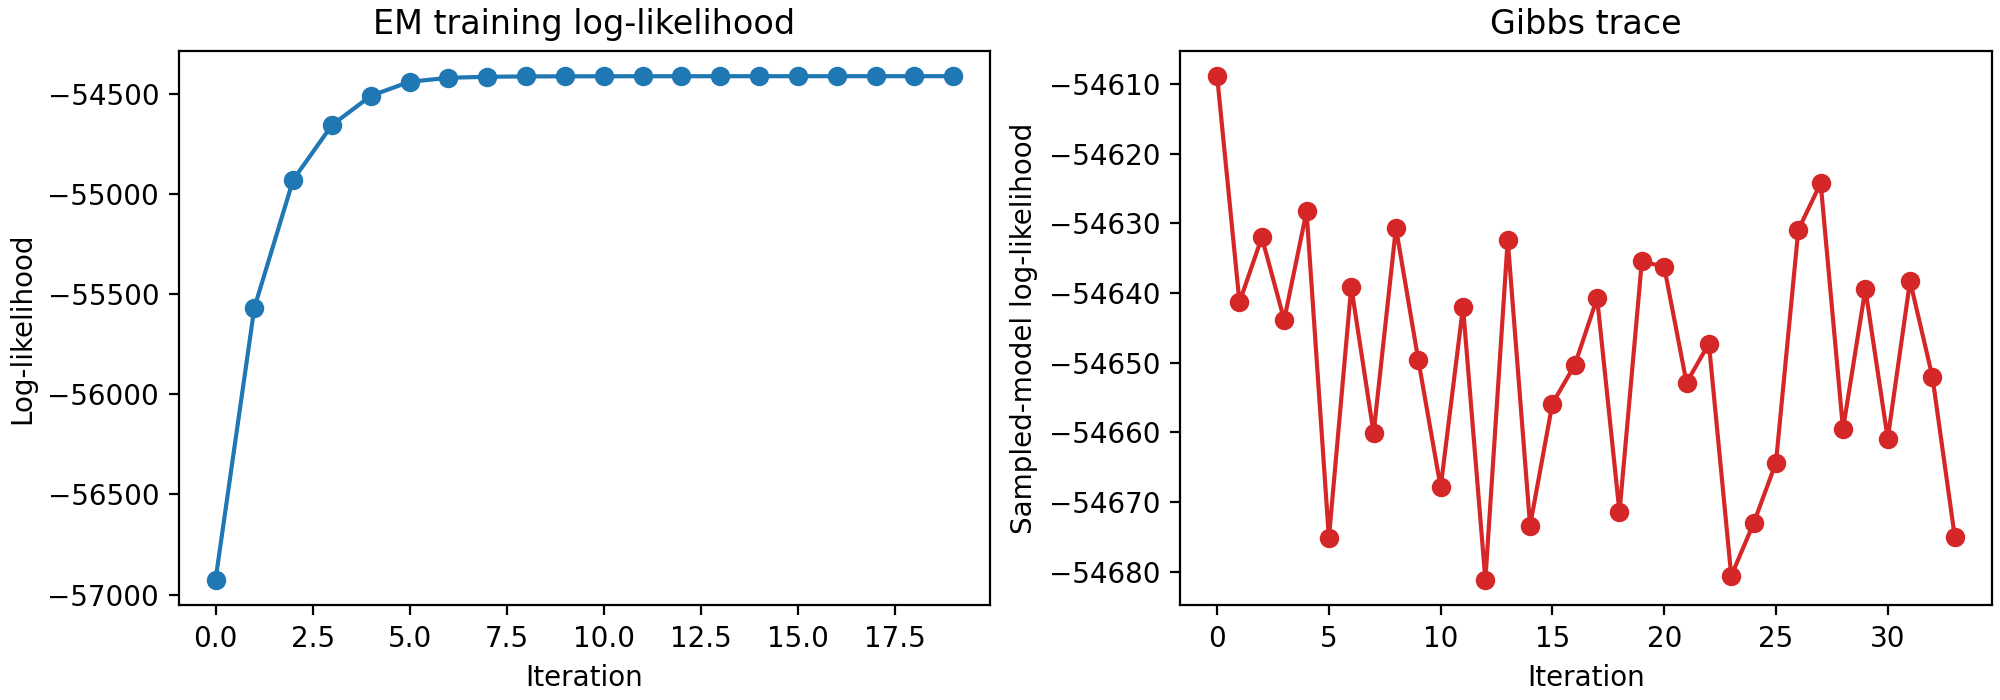
\includegraphics[width=\linewidth]{figures/convergence_diagnostics.png}
\caption{Optimization and sampling diagnostics. Left: EM training log-likelihood. Right: Bayesian sampled-model log-likelihood trace.}
\end{figure}

\begin{figure}[H]
\centering
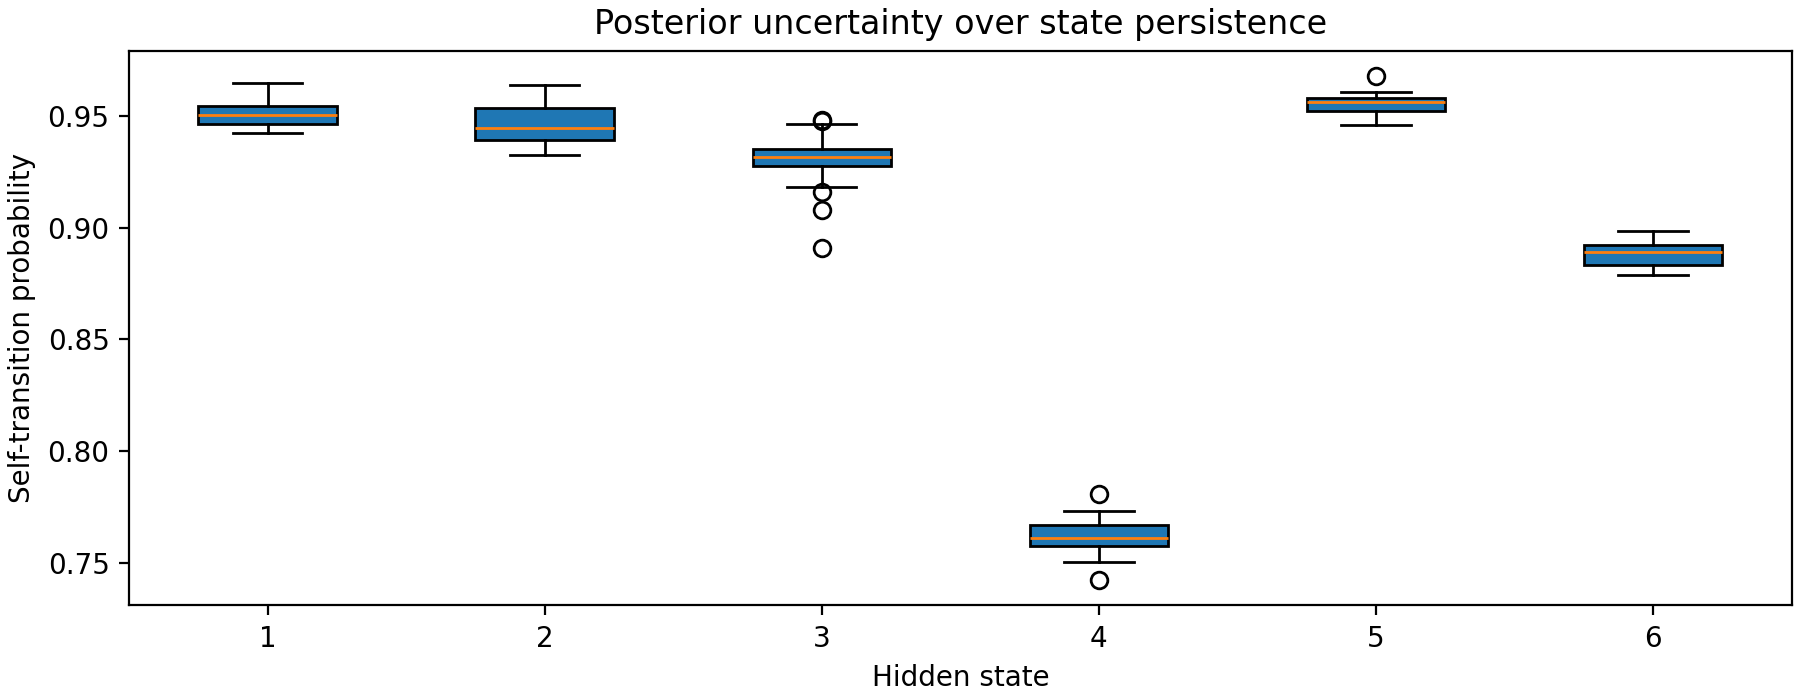
\includegraphics[width=0.88\linewidth]{figures/posterior_uncertainty.png}
\caption{Posterior uncertainty over diagonal entries of the transition matrix, illustrating variation in state persistence across posterior samples.}
\end{figure}

The noise-robustness experiment further shows how clustering quality changes after adding isotropic Gaussian noise in the PCA space. EM-HMM reached noisy-test ARI 0.298, whereas the Bayesian HMM reached 0.294.

\section{Discussion}
The Bayesian model adds meaningful interpretability even when its raw clustering metrics are close to the EM baseline. Instead of a single point estimate for transition structure, it yields a posterior over state persistence and transition uncertainty. This matters for HAR because some activities, such as sitting or laying, tend to persist for long runs, while motion classes transition more frequently.

At the same time, this project also exposed a practical limitation: fully Bayesian inference is more computationally expensive and more sensitive to initialization than EM. Our implementation therefore uses PCA-reduced features and conjugate priors to keep inference tractable. A stronger extension would be to replace the finite-state model with an HDP-HMM or to use the raw inertial signals directly with a structured emission model.

\section{Related Work}
Rabiner (1989) remains the standard reference for HMM inference and learning, especially the forward-backward and Baum-Welch algorithms. Scott (2002) studied Bayesian inference for HMMs with MCMC, showing how posterior sampling provides a richer picture of latent-state uncertainty than maximum likelihood alone. Beal (2003) developed variational Bayesian methods for graphical models, including HMMs, offering an alternative to sampling-based Bayesian inference. Teh et al. (2006) and Fox et al. (2008) extended Bayesian HMMs to nonparametric settings where the number of hidden states can be learned rather than fixed in advance. In the HAR domain, Anguita et al. (2013) introduced the benchmark smartphone dataset that we use here, though most follow-up work on this dataset has emphasized supervised discriminative models rather than unsupervised sequential Bayesian modeling.

\section{Conclusion}
This project demonstrates that a Bayesian Gaussian HMM is a feasible unsupervised model for smartphone-based HAR and that exact state inference plus Gibbs sampling can be implemented with standard conjugate updates. The toy-data experiment validates the inference pipeline, and the UCI HAR comparison shows that sequential probabilistic models can recover meaningful activity structure even without labels. The main gain from the Bayesian approach is not only performance, but also access to posterior uncertainty over transitions and emissions.

\begin{thebibliography}{9}
\bibitem{rabiner1989} L. R. Rabiner. A tutorial on hidden Markov models and selected applications in speech recognition. \textit{Proceedings of the IEEE}, 1989.
\bibitem{scott2002} S. L. Scott. Bayesian methods for hidden Markov models. \textit{Journal of the American Statistical Association}, 2002.
\bibitem{beal2003} M. J. Beal. Variational algorithms for approximate Bayesian inference. PhD thesis, University College London, 2003.
\bibitem{teh2006} Y. W. Teh, M. I. Jordan, M. J. Beal, and D. M. Blei. Hierarchical Dirichlet Processes. \textit{Journal of the American Statistical Association}, 2006.
\bibitem{fox2008} E. B. Fox, E. B. Sudderth, M. I. Jordan, and A. S. Willsky. An HDP-HMM for systems with state persistence. \textit{ICML}, 2008.
\bibitem{anguita2013} D. Anguita, A. Ghio, L. Oneto, X. Parra, and J. L. Reyes-Ortiz. A public domain dataset for human activity recognition using smartphones. \textit{ESANN}, 2013.
\end{thebibliography}

\end{document}
